\section{Experimentación}
El objetivo del trabajo era encontrar el \textit{mejor} arquero usando técnicas de métodos
numéricos. Qué dice qué arquero es mejor que otro es difícil de decidir cuando existen arqueros que
atajan tiros distintos pero en total la misma cantidad. En esta sección trataremos de decidir
utilizando los siguientes criterios:
%\begin{compactitem}
  %\item Diferencia en posición final: este criterio mide la distancia final entre la pelota y
    %nuestro arquero. Si es menor a 7 entonces nuestro arquero la atajó. Además, nos sirve para ir
    %analizando en el tiempo cómo es el comportamiento de nuestro arquero. \\
    %Los archivos de tests correspondientes son los que contienen al substring ".movsgol".
  %\item Diferencia en coordenada \texttr{y} a lo largo del tiempo: en este caso iremos viendo sólo la
    %información del eje \texttr{y} para cada momento de tiempo y comparándola en el caso de la pelota
    %y nuestro arquero. Nos sirve para ver cómo es el movimiento de nuestro arquero según se va
    %moviendo la pelota. Una estrategia \textrt{ingenua} que no consideramos en nuestro trabajo sería
    %ir acercando el arquero a cada coordenada \texttt{y} de la pelota a lo largo del tiempo, sin
    %considerar que pueda cambiar bruscamente y nos alejemos demasiado del destino final.
    %\\
    %Los archivos de tests correspondientes son los que contienen al substring ".movstodos".
  %\item Error en estimación: compara la posición de gol de la pelota contra la estimación de
    %nuestros métodos. Es decir, en cada momento qué tan errada está la estimación de por dónde va a
    %entrar la pelota. Sirve para ver cómo va cambiando la estimación con más información o mientras
    %más se acerca al arco.
    %\\
  %  Los archivos de tests correspondientes son los que contienen al substring ".movsestimacion".
 % \end{compactitem}


\section{Resultados}


\subsection{Experimentación con Lineales}

\textbf{Utilizando lineal6.tiro}

\begin{figure}[H]
\begin{center}
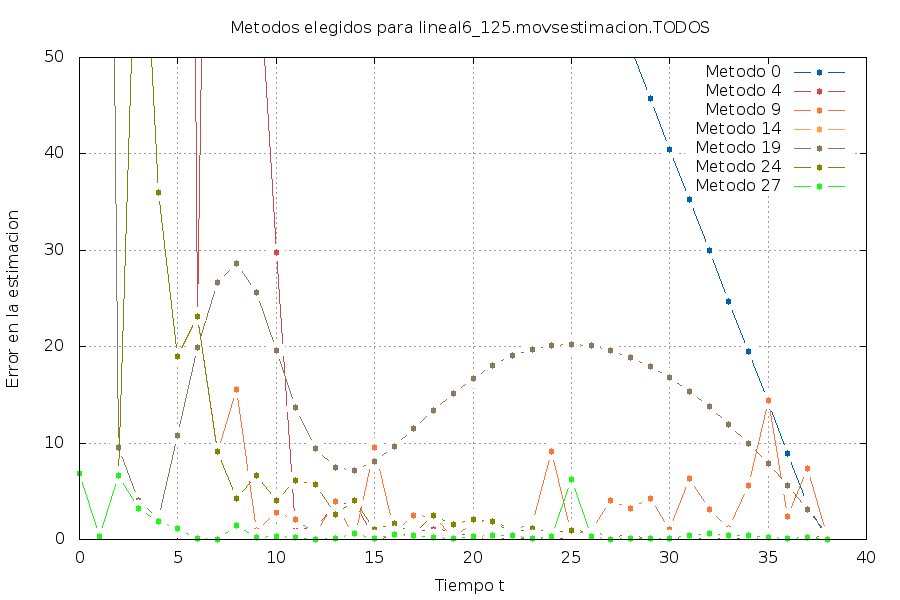
\includegraphics[width=0.9\textwidth]{img/lineal6_125_movsestimacion_TODOS_elegidos.png}
     \caption{ESTIMACION de tiro lineal6}
\end{center}
\end{figure}

\begin{figure}[H]
\begin{center}
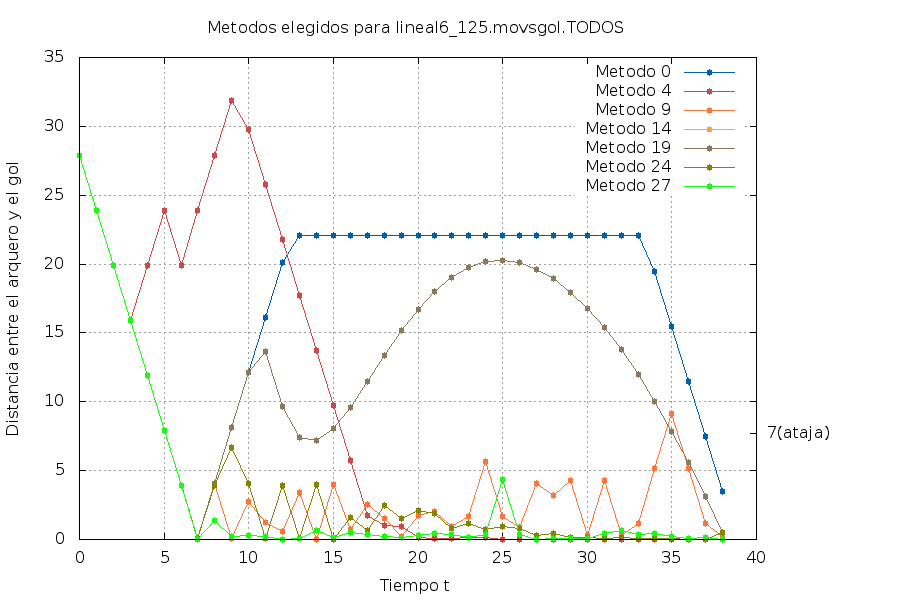
\includegraphics[width=0.9\textwidth]{img/lineal6_125_movsgol_TODOS_elegidos.png}
     \caption{MOVSGOL de tiro lineal6}
\end{center}
\end{figure}


\begin{figure}[H]
\begin{center}
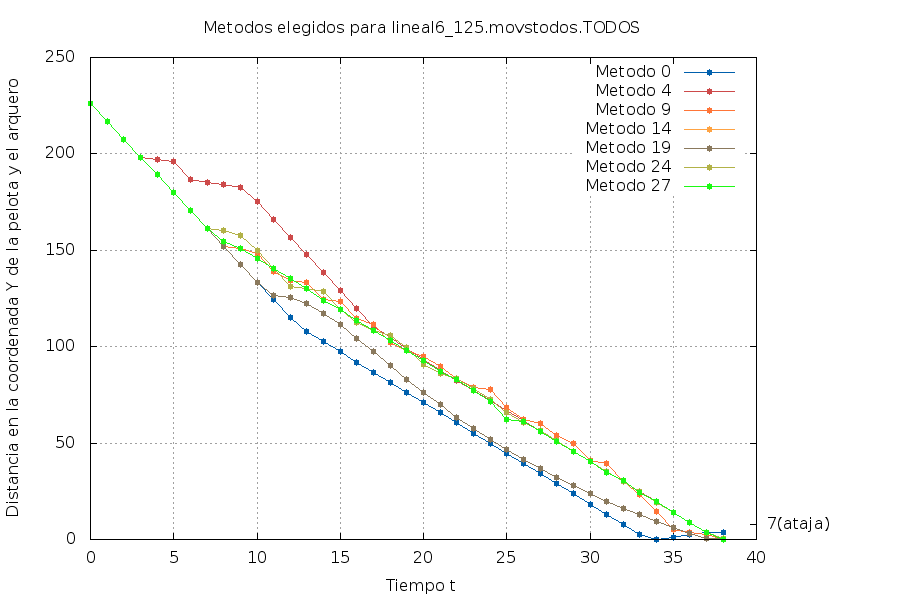
\includegraphics[width=0.9\textwidth]{img/lineal6_125_movstodos_TODOS_elegidos.png}
     \caption{MOVSTODOS de tiro lineal6}
\end{center}
\end{figure}

\subsubsection{Concluciones}
\subsection{Experimentacion con Curvas}

\textbf{Utilizando cuadr3.tiro}

\begin{figure}[H]
\begin{center}
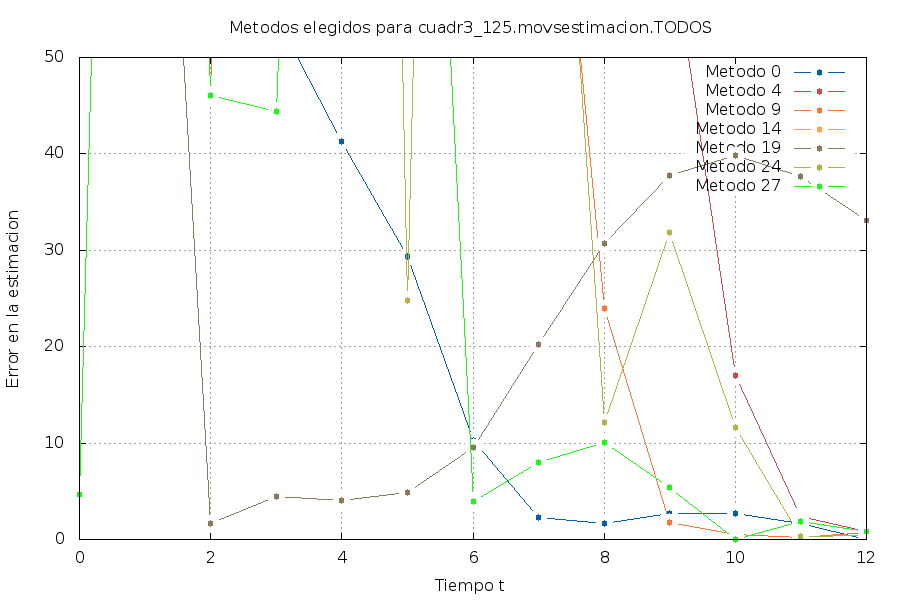
\includegraphics[width=0.9\textwidth]{img/cuadr3_125_movsestimacion_TODOS_elegidos.png}
     \caption{Estimacion de tiro cuadr3}
\end{center}
\end{figure}

\begin{figure}[H]
\begin{center}
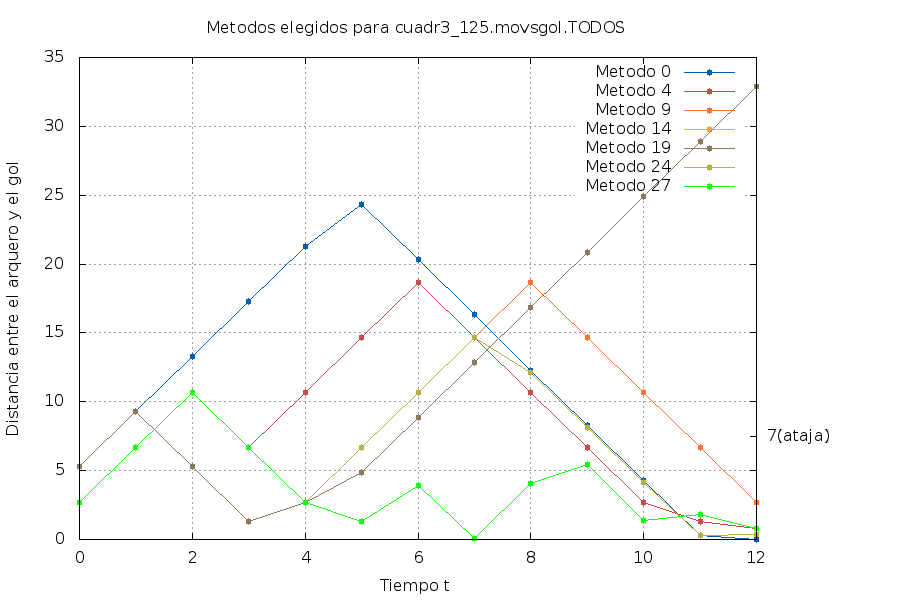
\includegraphics[width=0.9\textwidth]{img/cuadr3_125_movsgol_TODOS_elegidos.png}
     \caption{MOVSGOL de tiro cuadr3}
\end{center}
\end{figure}


\begin{figure}[H]
\begin{center}
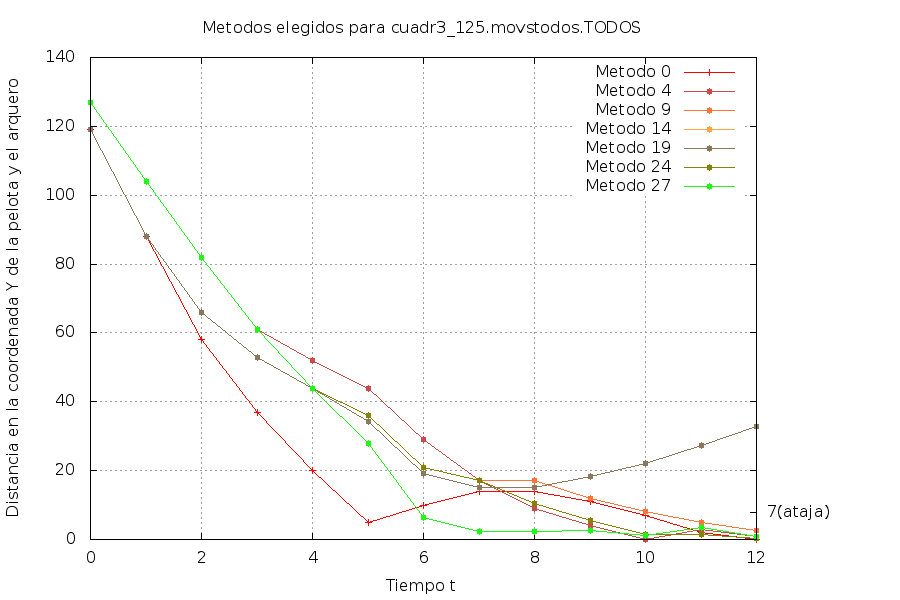
\includegraphics[width=0.9\textwidth]{img/cuadr3_125_movstodos_TODOS_elegidos.png}
     \caption{MOVSTODOS de tiro cuadr3}
\end{center}
\end{figure}

\textbf{Utilizando cuadr6.tiro}

\begin{figure}[H]
\begin{center}
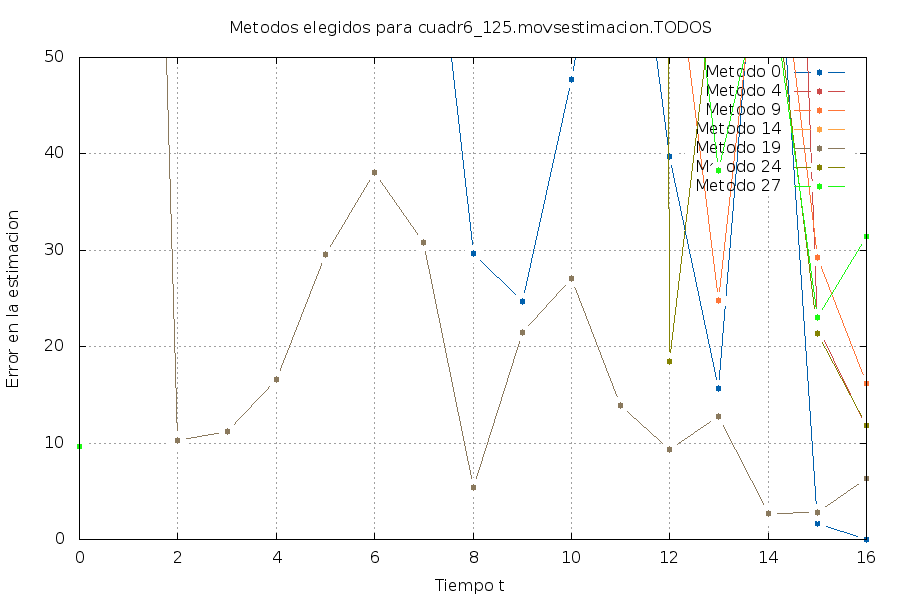
\includegraphics[width=0.9\textwidth]{img/cuadr6_125_movsestimacion_TODOS_elegidos.png}
     \caption{Estimacion de tiro cuadr6}
\end{center}
\end{figure}

\begin{figure}[H]
\begin{center}
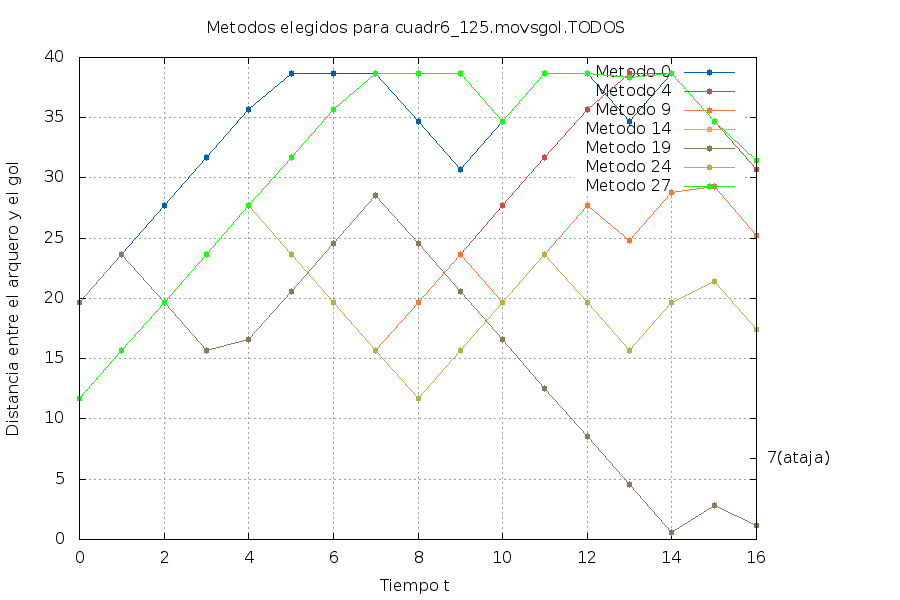
\includegraphics[width=0.9\textwidth]{img/cuadr6_125_movsgol_TODOS_elegidos.png}
     \caption{MOVSGOL de tiro cuadr6}
\end{center}
\end{figure}

\begin{figure}[H]
\begin{center}
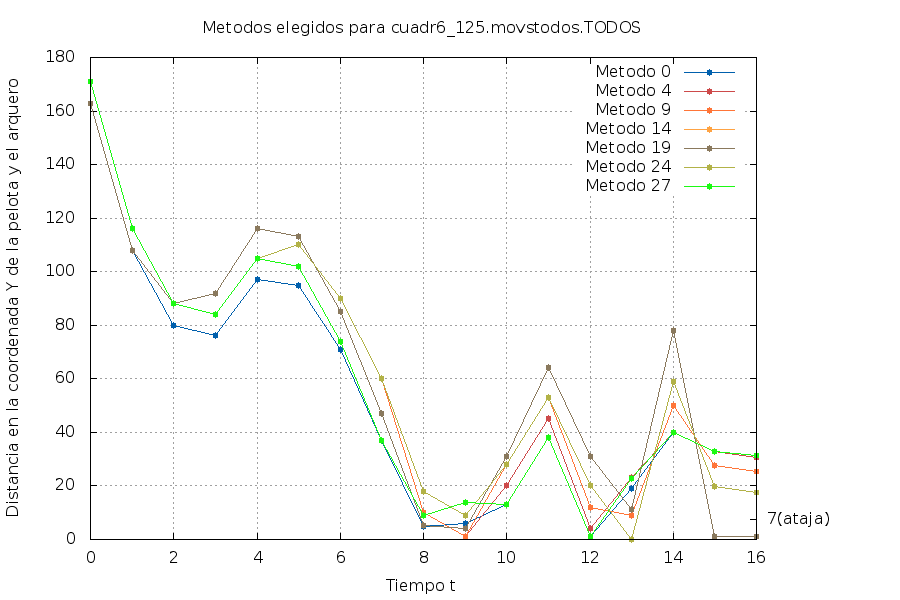
\includegraphics[width=0.9\textwidth]{img/cuadr6_125_movstodos_TODOS_elegidos.png}
     \caption{MOVSTODOS de tiro cuadr6}
\end{center}     
\end{figure}

\subsubsection{Concluciones}

\subsection{Experimentacion con Jugadores}


\textbf{Utilizando conj4.tiro}

\begin{figure}[H]
\begin{center}
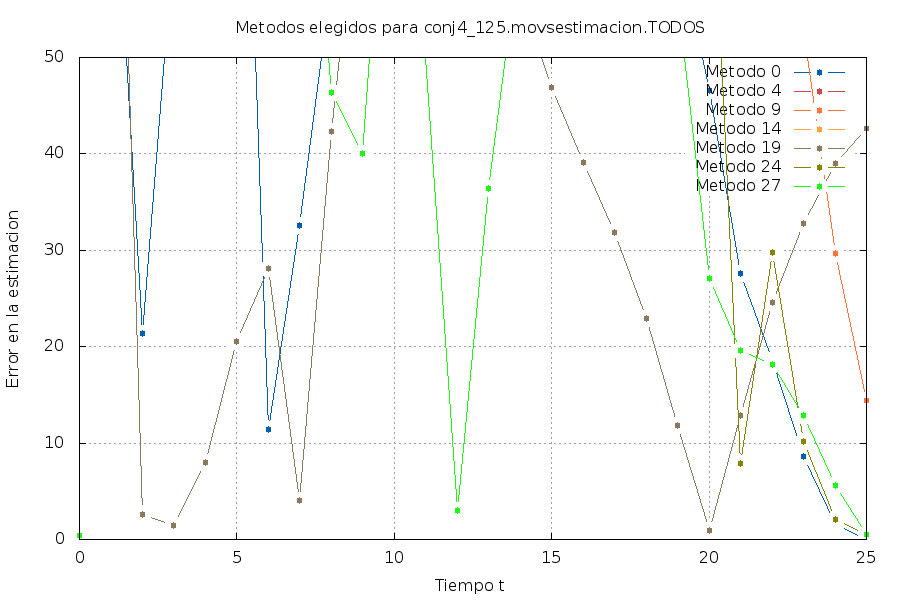
\includegraphics[width=0.9\textwidth]{img/conj4_125_movsestimacion_TODOS_elegidos.png}
     \caption{Estimacion de tiro conj4}
\end{center}
\end{figure}

\begin{figure}[H]
\begin{center}
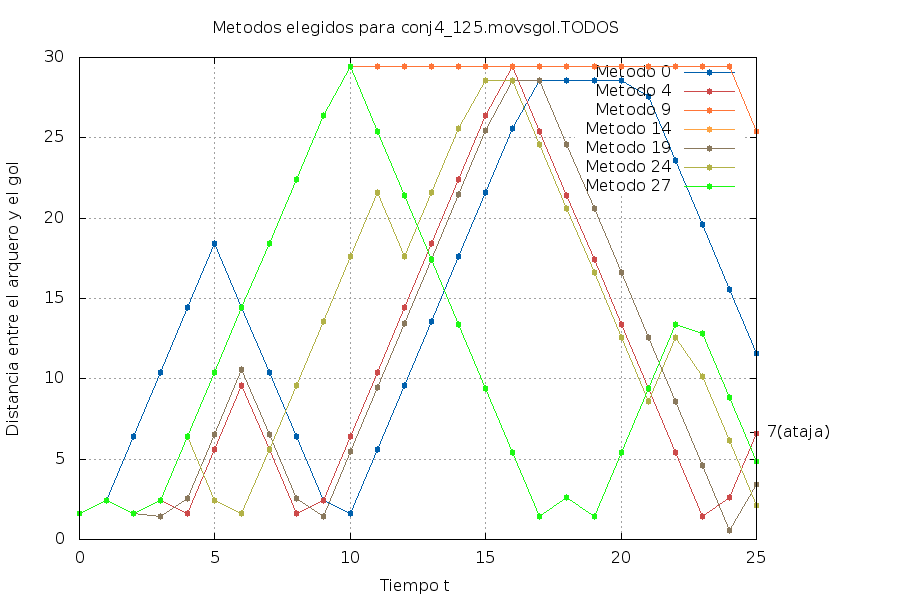
\includegraphics[width=0.9\textwidth]{img/conj4_125_movsgol_TODOS_elegidos.png}
     \caption{MOVSGOL de tiro conj4}
\end{center}
\end{figure}

\begin{figure}[H]
\begin{center}
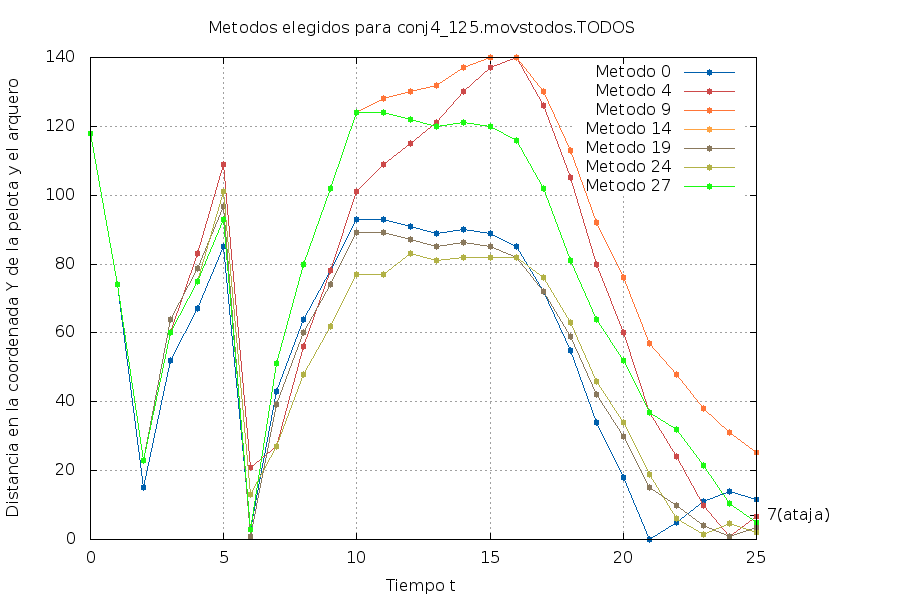
\includegraphics[width=0.9\textwidth]{img/conj4_125_movstodos_TODOS_elegidos.png}
     \caption{MOVSTODOS de tiro conj4}
\end{center}
\end{figure}



\textbf{Utilizando conj8.tiro}

\begin{figure}[H]
\begin{center}
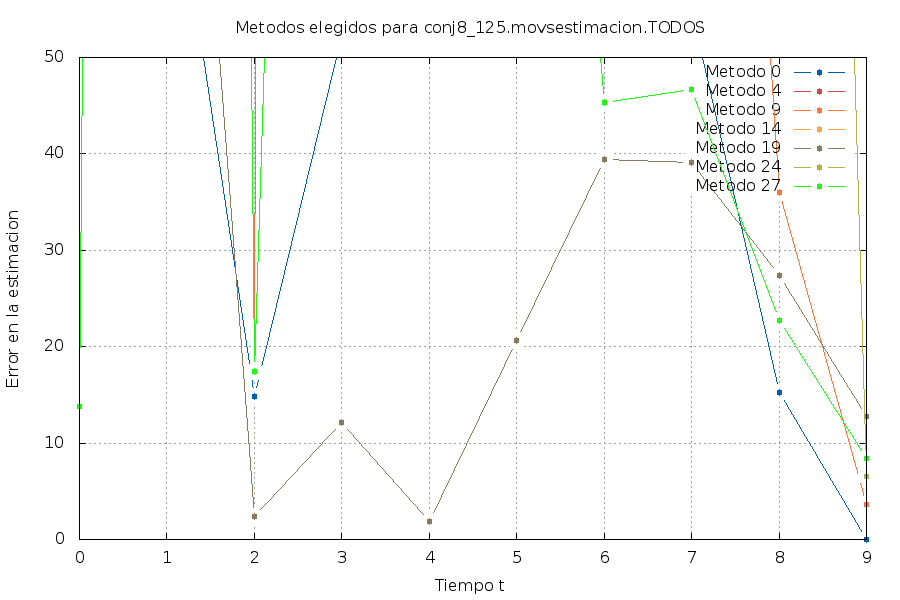
\includegraphics[width=0.9\textwidth]{img/conj8_125_movsestimacion_TODOS_elegidos.png}
     \caption{Estimacion de tiro conj8}
\end{center}
\end{figure}

\begin{figure}[H]
\begin{center}
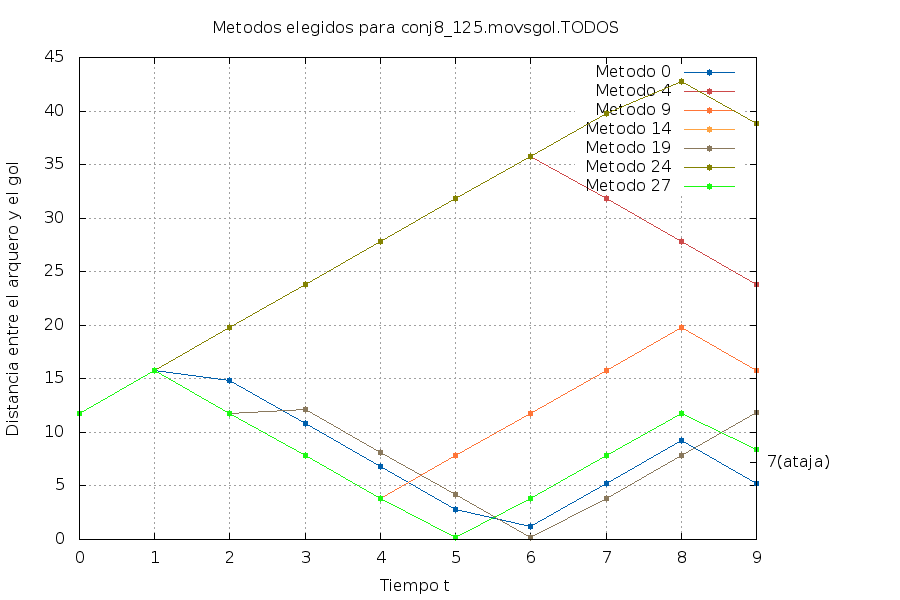
\includegraphics[width=0.9\textwidth]{img/conj8_125_movsgol_TODOS_elegidos.png}
     \caption{MOVSGOL de tiro conj8}
\end{center}
\end{figure}

\begin{figure}[H]
\begin{center}
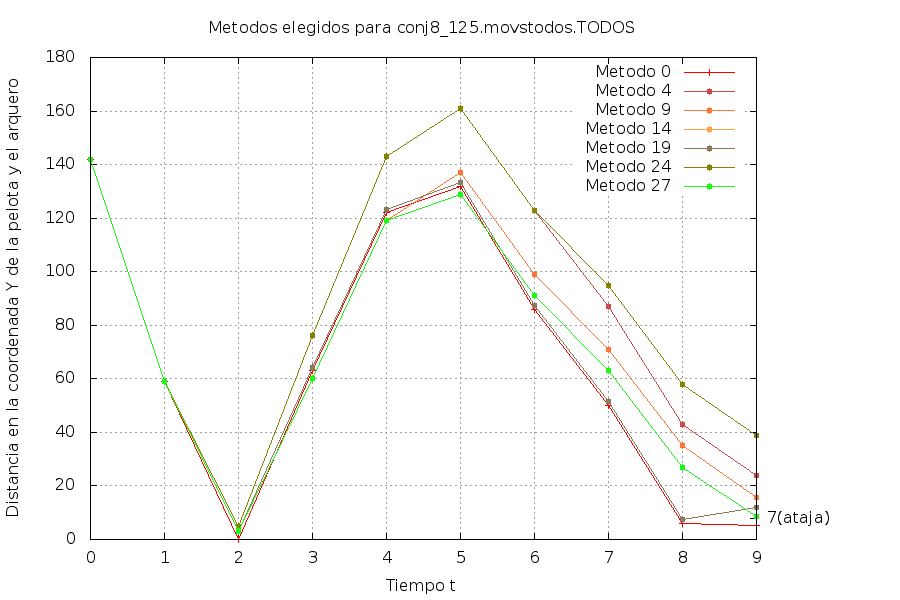
\includegraphics[width=0.9\textwidth]{img/conj8_125_movstodos_TODOS_elegidos.png}
     \caption{MOVSTODOS de tiro conj8}
\end{center}
\end{figure}


\subsubsection{Concluciones}

\subsection{Experimentacion con Exoticos}

\textbf{Utilizando ex5.tiro}

\begin{figure}[H]
\begin{center}
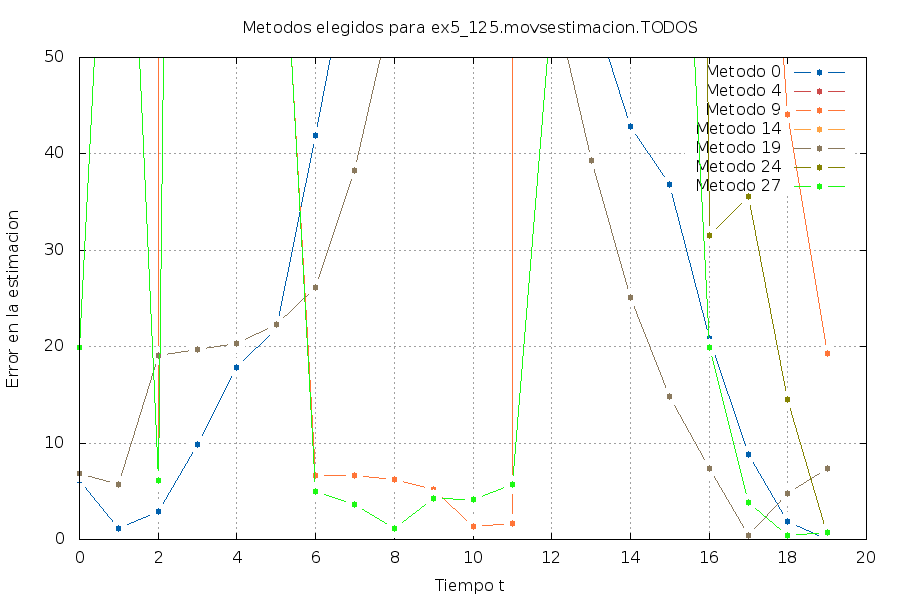
\includegraphics[width=0.9\textwidth]{img/ex5_125_movsestimacion_TODOS_elegidos.png}
     \caption{Estimacion de tiro ex5}
\end{center}
\end{figure}

\begin{figure}[H]
\begin{center}
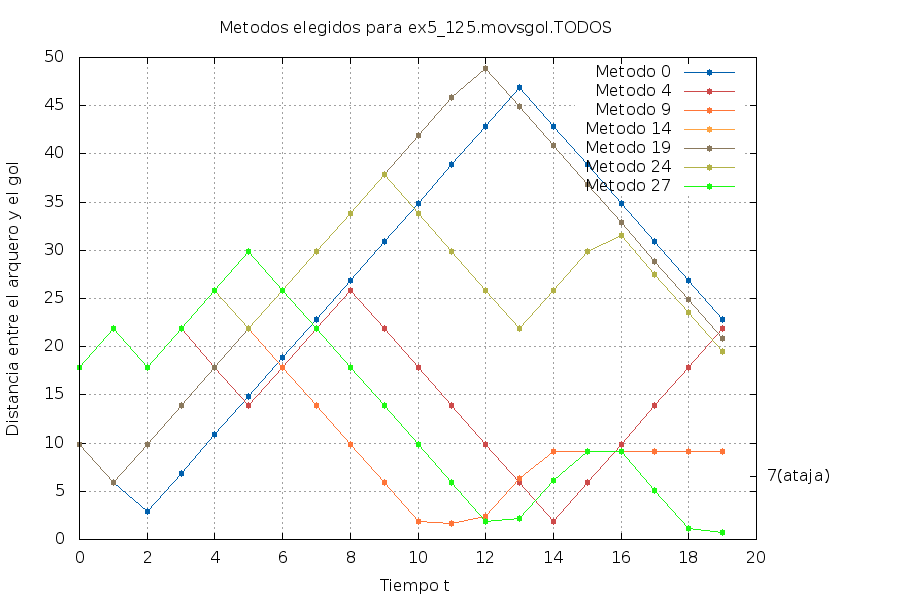
\includegraphics[width=0.9\textwidth]{img/ex5_125_movsgol_TODOS_elegidos.png}
     \caption{MOVSGOL de tiro ex5}
\end{center}
\end{figure}

\begin{figure}[H]
\begin{center}
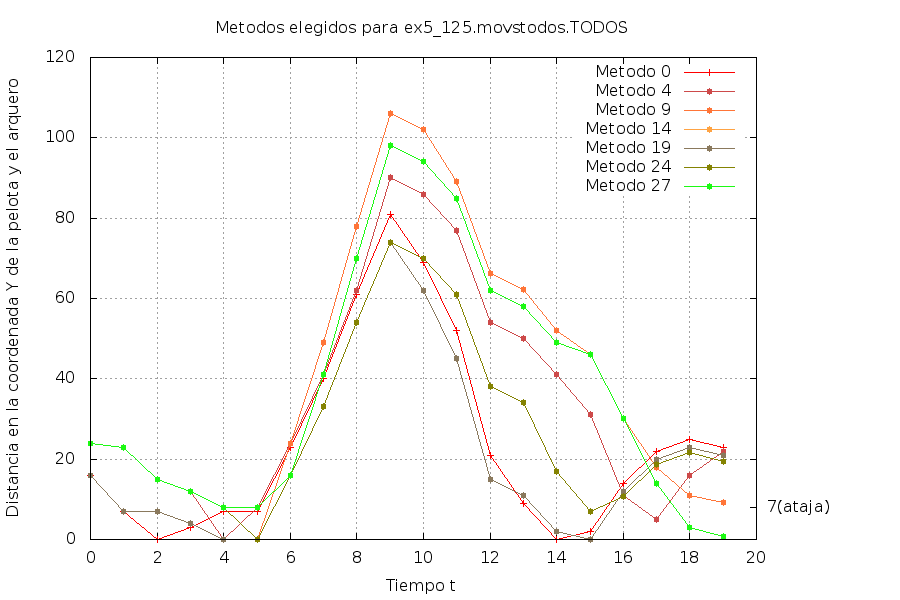
\includegraphics[width=0.9\textwidth]{img/ex5_125_movstodos_TODOS_elegidos.png}
     \caption{MOVSTODOS de tiro ex5}
\end{center}
\end{figure}


\subsubsection{Concluciones}

\subsection{Concluciones Finales}
